\documentclass[12pt,letterpaper]{article}
\usepackage{graphicx,textcomp}
\usepackage{natbib}
\usepackage{setspace}
\usepackage{fullpage}
\usepackage{color}
\usepackage[reqno]{amsmath}
\usepackage{amsthm}
\usepackage{fancyvrb}
\usepackage{amssymb,enumerate}
\usepackage[all]{xy}
\usepackage{endnotes}
\usepackage{lscape}
\newtheorem{com}{Comment}
\usepackage{float}
\usepackage{hyperref}
\newtheorem{lem} {Lemma}
\newtheorem{prop}{Proposition}
\newtheorem{thm}{Theorem}
\newtheorem{defn}{Definition}
\newtheorem{cor}{Corollary}
\newtheorem{obs}{Observation}
\usepackage[compact]{titlesec}
\usepackage{dcolumn}
\usepackage{tikz}
\usetikzlibrary{arrows}
\usepackage{multirow}
\usepackage{subcaption}
\usepackage{xcolor}
\newcolumntype{.}{D{.}{.}{-1}}
\newcolumntype{d}[1]{D{.}{.}{#1}}
\definecolor{light-gray}{gray}{0.65}
\usepackage{url}
\usepackage{listings}
\usepackage{color}

\definecolor{codegreen}{rgb}{0,0.6,0}
\definecolor{codegray}{rgb}{0.5,0.5,0.5}
\definecolor{codepurple}{rgb}{0.58,0,0.82}
\definecolor{backcolour}{rgb}{0.95,0.95,0.92}

\lstdefinestyle{mystyle}{
	backgroundcolor=\color{backcolour},   
	commentstyle=\color{codegreen},
	keywordstyle=\color{magenta},
	numberstyle=\tiny\color{codegray},
	stringstyle=\color{codepurple},
	basicstyle=\footnotesize,
	breakatwhitespace=false,         
	breaklines=true,                 
	captionpos=b,                    
	keepspaces=true,                 
	numbers=left,                    
	numbersep=5pt,                  
	showspaces=false,                
	showstringspaces=false,
	showtabs=false,                  
	tabsize=2
}
\lstset{style=mystyle}
\newcommand{\Sref}[1]{Section~\ref{#1}}

\title{PS01 Response}
\date{Zach Keller}
\author{Applied Stats/Quant Methods 1}

\begin{document}
	\maketitle
	


\section*{Question 1 }

\vspace{.25cm}

\noindent First, the data was explored. Both histograms and QQ plots were created to determine whether to use T scores or Z scores by investigating whether the data is normal \\ 

\begin{figure}[h!]\centering
	\caption{\footnotesize Histogram of IQ Scores.}
	\label{fig:plot_1}
	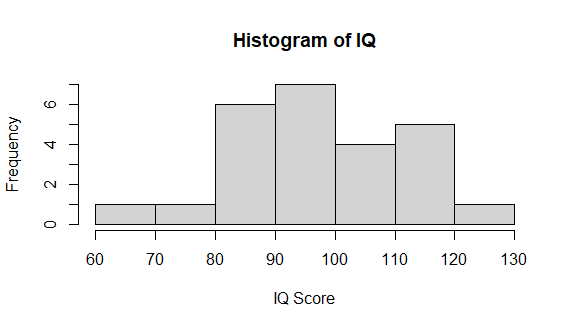
\includegraphics[width=.75\textwidth]{iqhist.png}
\end{figure} 

\begin{figure}[h!]\centering
	\caption{\footnotesize QQ Plot of IQ Scores.}
	\label{fig:plot_1}
	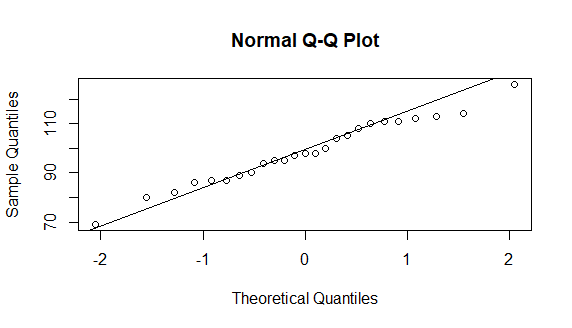
\includegraphics[width=.75\textwidth]{qqplotiq.png}
\end{figure}

\begin{figure}[h!]\centering
	\caption{\footnotesize Plot Density Plot of IQ Scores.}
	\label{fig:plot_1}
	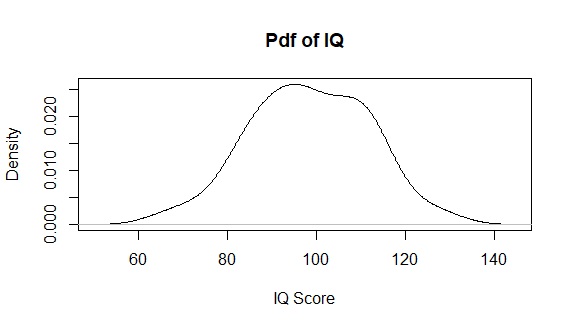
\includegraphics[width=.75\textwidth]{pdfiq.png}
\end{figure}
\vspace{.25cm}

\noindent As shown above, the data does not look to be normally distributed. Therefore, it was decided that T Scores were more suitable to use. More specifically, a one-tailed one-sampled t-test was used, as we are only testing in one direction. In order to construct a confidence interval, the following code was used:\\

\lstinputlisting[language=R, firstline=66, lastline=69]{code/PS01.R} 
\vspace{.5cm}

\noindent From this code, it was calculated that the confidence interval was that the mean was between 93.96 and 102.92. This was confirmed when running the data through the t-test function\\
\vspace{.25cm}

\begin{verbatim}
	One Sample t-test
	
	data:  y
	t = 37.593, df = 24, p-value < 2.2e-16
	alternative hypothesis: true mean is not equal to 0
	90 percent confidence interval:
	93.95993 102.92007
	sample estimates:
	mean of x 
	98.44 
\end{verbatim}


\noindent Now for the hypothesis test. The first step involves making assumptions about your data. As shown from the data visualisations in the last part, the data is not normally distributed and has a small sample size. Step two involves creating your null and alternative hypotheses. In this case, the hypotheses would be as follows:\\

\lstinputlisting[language=R, firstline=84, lastline=85]{code/PS01.R} 
\vspace{.5cm}

\noindent Step three is the test statistic, which was obtained from the the following code, which produced the results below:

\begin{verbatim}
> t.test(y, conf.level = 0.95, alternative = "greater", mu = 100)

One Sample t-test

data:  y
t = -0.59574, df = 24, p-value = 0.7215
alternative hypothesis: true mean is greater than 100
95 percent confidence interval:
93.95993      Inf
sample estimates:
mean of x 
98.44 
\end{verbatim}

\noindent This \textit{p} value is greater than .05, meaning we fail to reject the null hypothesis. This implies that the sample mean is either less than or equal to 100, the population mean for IQ Scores.\\

\section*{Question 2}  

\begin{figure}[h!]\centering
	\caption{\footnotesize Required Graphs.}
	\label{fig:plots}
	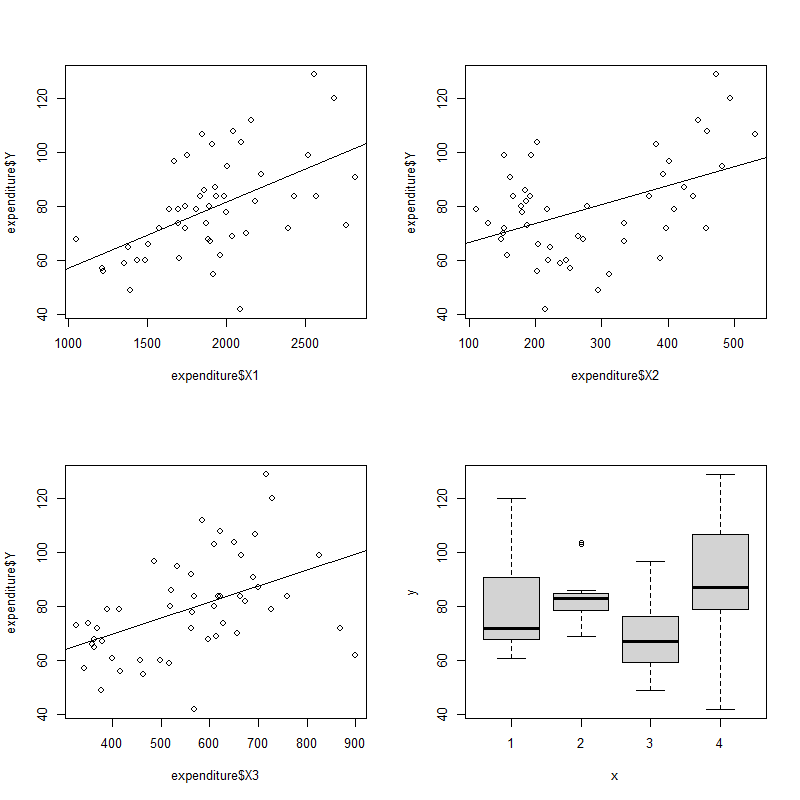
\includegraphics[width=.75\textwidth]{Rplot01.png}
\end{figure}

\noindent Figure 4 contains three scatterplots which show the relationships between Y and the different X variables.\\

\noindent All of these scatterplots display a positive relationship, with the sample slope being positive on all tables. However, these relationships would be considered moderate, with the above data having correlations of \textit{r} = .53, \textit{r} = .44, and \textit{r} = .46 respectively, which would be considered moderate correlations. This was done by calculating the square root of \textit{r} from Tables 1-3 shown below. \\

\noindent Also, the boxplot in Figure 4 displays that Region 4 has the highest mean spending compared to the other regions. \\


% Table created by stargazer v.5.2.3 by Marek Hlavac, Social Policy Institute. E-mail: marek.hlavac at gmail.com
% Date and time: Thu, Oct 13, 2022 - 13:19:09
\begin{table}[!htbp] \centering 
  \caption{} 
  \label{} 
\begin{tabular}{@{\extracolsep{5pt}}lc} 
\\[-1.8ex]\hline 
\hline \\[-1.8ex] 
 & \multicolumn{1}{c}{\textit{Dependent variable:}} \\ 
\cline{2-2} 
\\[-1.8ex] & water \\ 
\hline \\[-1.8ex] 
 irrigation & 1.445$^{***}$ \\ 
  & (0.181) \\ 
  & \\ 
 Constant & 13.125$^{***}$ \\ 
  & (1.816) \\ 
  & \\ 
\hline \\[-1.8ex] 
Observations & 322 \\ 
R$^{2}$ & 0.166 \\ 
Adjusted R$^{2}$ & 0.163 \\ 
Residual Std. Error & 30.806 (df = 320) \\ 
F Statistic & 63.655$^{***}$ (df = 1; 320) \\ 
\hline 
\hline \\[-1.8ex] 
\textit{Note:}  & \multicolumn{1}{r}{$^{*}$p$<$0.1; $^{**}$p$<$0.05; $^{***}$p$<$0.01} \\ 
\end{tabular} 
\end{table}  

% Table created by stargazer v.5.2.3 by Marek Hlavac, Social Policy Institute. E-mail: marek.hlavac at gmail.com
% Date and time: Thu, Oct 13, 2022 - 13:30:29
\begin{table}[!htbp] \centering 
  \caption{} 
  \label{} 
\begin{tabular}{@{\extracolsep{5pt}}lc} 
\\[-1.8ex]\hline 
\hline \\[-1.8ex] 
 & \multicolumn{1}{c}{\textit{Dependent variable:}} \\ 
\cline{2-2} 
\\[-1.8ex] & water \\ 
\hline \\[-1.8ex] 
 irrigation & 1.454$^{***}$ \\ 
  & (0.180) \\ 
  & \\ 
 female1 & 8.412$^{**}$ \\ 
  & (3.503) \\ 
  & \\ 
 Constant & 9.858$^{***}$ \\ 
  & (2.258) \\ 
  & \\ 
\hline \\[-1.8ex] 
Observations & 322 \\ 
R$^{2}$ & 0.181 \\ 
Adjusted R$^{2}$ & 0.176 \\ 
Residual Std. Error & 30.579 (df = 319) \\ 
F Statistic & 35.186$^{***}$ (df = 2; 319) \\ 
\hline 
\hline \\[-1.8ex] 
\textit{Note:}  & \multicolumn{1}{r}{$^{*}$p$<$0.1; $^{**}$p$<$0.05; $^{***}$p$<$0.01} \\ 
\end{tabular} 
\end{table}  

% Table created by stargazer v.5.2.3 by Marek Hlavac, Social Policy Institute. E-mail: marek.hlavac at gmail.com
% Date and time: Thu, Oct 13, 2022 - 15:00:23
\begin{table}[!htbp] \centering 
  \caption{} 
  \label{} 
\begin{tabular}{@{\extracolsep{5pt}}lc} 
\\[-1.8ex]\hline 
\hline \\[-1.8ex] 
 & \multicolumn{1}{c}{\textit{Dependent variable:}} \\ 
\cline{2-2} 
\\[-1.8ex] & water \\ 
\hline \\[-1.8ex] 
 irrigation & 0.958$^{***}$ \\ 
  & (0.187) \\ 
  & \\ 
 female1 & $-$0.258 \\ 
  & (3.584) \\ 
  & \\ 
 irrigation:female1 & 2.798$^{***}$ \\ 
  & (0.445) \\ 
  & \\ 
 Constant & 11.547$^{***}$ \\ 
  & (2.150) \\ 
  & \\ 
\hline \\[-1.8ex] 
Observations & 322 \\ 
R$^{2}$ & 0.271 \\ 
Adjusted R$^{2}$ & 0.264 \\ 
Residual Std. Error & 28.884 (df = 318) \\ 
F Statistic & 39.472$^{***}$ (df = 3; 318) \\ 
\hline 
\hline \\[-1.8ex] 
\textit{Note:}  & \multicolumn{1}{r}{$^{*}$p$<$0.1; $^{**}$p$<$0.05; $^{***}$p$<$0.01} \\ 
\end{tabular} 
\end{table}  

% Table created by stargazer v.5.2.3 by Marek Hlavac, Social Policy Institute. E-mail: marek.hlavac at gmail.com
% Date and time: Thu, Oct 13, 2022 - 15:01:15
\begin{table}[!htbp] \centering 
  \caption{} 
  \label{} 
\begin{tabular}{@{\extracolsep{5pt}}lc} 
\\[-1.8ex]\hline 
\hline \\[-1.8ex] 
 & \multicolumn{1}{c}{\textit{Dependent variable:}} \\ 
\cline{2-2} 
\\[-1.8ex] & water \\ 
\hline \\[-1.8ex] 
 irrigation & 0.958$^{***}$ \\ 
  & (0.187) \\ 
  & \\ 
 female1 & $-$0.258 \\ 
  & (3.584) \\ 
  & \\ 
 irrigation:female1 & 2.798$^{***}$ \\ 
  & (0.445) \\ 
  & \\ 
 Constant & 11.547$^{***}$ \\ 
  & (2.150) \\ 
  & \\ 
\hline \\[-1.8ex] 
Observations & 322 \\ 
R$^{2}$ & 0.271 \\ 
Adjusted R$^{2}$ & 0.264 \\ 
Residual Std. Error & 28.884 (df = 318) \\ 
F Statistic & 39.472$^{***}$ (df = 3; 318) \\ 
\hline 
\hline \\[-1.8ex] 
\textit{Note:}  & \multicolumn{1}{r}{$^{*}$p$<$0.1; $^{**}$p$<$0.05; $^{***}$p$<$0.01} \\ 
\end{tabular} 
\end{table}  

% Table created by stargazer v.5.2.3 by Marek Hlavac, Social Policy Institute. E-mail: marek.hlavac at gmail.com
% Date and time: Sun, Oct 16, 2022 - 21:30:13
\begin{table}[!htbp] \centering 
  \caption{} 
  \label{} 
\begin{tabular}{@{\extracolsep{5pt}}lc} 
\\[-1.8ex]\hline 
\hline \\[-1.8ex] 
 & \multicolumn{1}{c}{\textit{Dependent variable:}} \\ 
\cline{2-2} 
\\[-1.8ex] & water \\ 
\hline \\[-1.8ex] 
 reserved1 & 9.252$^{**}$ \\ 
  & (3.948) \\ 
  & \\ 
 Constant & 14.738$^{***}$ \\ 
  & (2.286) \\ 
  & \\ 
\hline \\[-1.8ex] 
Observations & 322 \\ 
R$^{2}$ & 0.017 \\ 
Adjusted R$^{2}$ & 0.014 \\ 
Residual Std. Error & 33.446 (df = 320) \\ 
F Statistic & 5.493$^{**}$ (df = 1; 320) \\ 
\hline 
\hline \\[-1.8ex] 
\textit{Note:}  & \multicolumn{1}{r}{$^{*}$p$<$0.1; $^{**}$p$<$0.05; $^{***}$p$<$0.01} \\ 
\end{tabular} 
\end{table}  


% Table created by stargazer v.5.2.3 by Marek Hlavac, Social Policy Institute. E-mail: marek.hlavac at gmail.com
% Date and time: Sun, Oct 02, 2022 - 16:25:43
\begin{table}[!htbp] \centering 
  \caption{} 
  \label{} 
\begin{tabular}{@{\extracolsep{5pt}}lc} 
\\[-1.8ex]\hline 
\hline \\[-1.8ex] 
 & \multicolumn{1}{c}{\textit{Dependent variable:}} \\ 
\cline{2-2} 
\\[-1.8ex] & Y \\ 
\hline \\[-1.8ex] 
 X2 & 0.070$^{***}$ \\ 
  & (0.020) \\ 
  & \\ 
 Constant & 59.761$^{***}$ \\ 
  & (6.164) \\ 
  & \\ 
\hline \\[-1.8ex] 
Observations & 50 \\ 
R$^{2}$ & 0.201 \\ 
Adjusted R$^{2}$ & 0.184 \\ 
Residual Std. Error & 16.714 (df = 48) \\ 
F Statistic & 12.072$^{***}$ (df = 1; 48) \\ 
\hline 
\hline \\[-1.8ex] 
\textit{Note:}  & \multicolumn{1}{r}{$^{*}$p$<$0.1; $^{**}$p$<$0.05; $^{***}$p$<$0.01} \\ 
\end{tabular} 
\end{table}  


% Table created by stargazer v.5.2.3 by Marek Hlavac, Social Policy Institute. E-mail: marek.hlavac at gmail.com
% Date and time: Sun, Oct 02, 2022 - 16:25:44
\begin{table}[!htbp] \centering 
  \caption{} 
  \label{} 
\begin{tabular}{@{\extracolsep{5pt}}lc} 
\\[-1.8ex]\hline 
\hline \\[-1.8ex] 
 & \multicolumn{1}{c}{\textit{Dependent variable:}} \\ 
\cline{2-2} 
\\[-1.8ex] & Y \\ 
\hline \\[-1.8ex] 
 X3 & 0.059$^{***}$ \\ 
  & (0.016) \\ 
  & \\ 
 Constant & 46.306$^{***}$ \\ 
  & (9.461) \\ 
  & \\ 
\hline \\[-1.8ex] 
Observations & 50 \\ 
R$^{2}$ & 0.215 \\ 
Adjusted R$^{2}$ & 0.199 \\ 
Residual Std. Error & 16.567 (df = 48) \\ 
F Statistic & 13.146$^{***}$ (df = 1; 48) \\ 
\hline 
\hline \\[-1.8ex] 
\textit{Note:}  & \multicolumn{1}{r}{$^{*}$p$<$0.1; $^{**}$p$<$0.05; $^{***}$p$<$0.01} \\ 
\end{tabular} 
\end{table}  


\noindent As previously shown in Table 1, Y and X1 have a moderate positive relationship, with the estimated slope being 0.025. The \textit{R} squared value is 0.283, meaning that the regression model can only account for 28.3 percent of the variability in the data.\\

\noindent The graph in Figure 5 displays the expenditure depending on the region, with each region being represented by a different colour, as shown by the key to the right of the graph.

\begin{figure}[h!]\centering
	\caption{\footnotesize Scatterplot of Y against X1}
	\label{fig:plots1}
	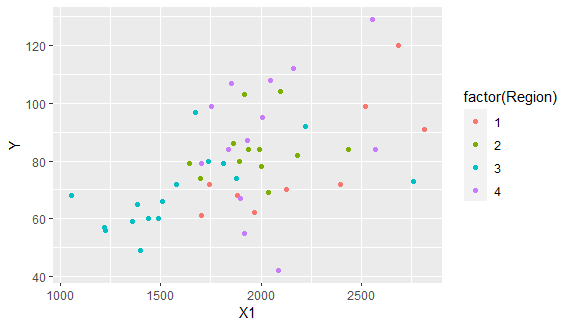
\includegraphics[width=.75\textwidth]{Rplot03.png}
\end{figure}


\end{document}
